%%%%%%%% ICML 2018 EXAMPLE LATEX SUBMISSION FILE %%%%%%%%%%%%%%%%%

\documentclass{article}

% Recommended, but optional, packages for figures and better typesetting:
\usepackage{microtype}
\usepackage{graphicx}
\usepackage{subfigure}
\usepackage{amsmath}
\usepackage{amssymb}
\usepackage{booktabs} % for professional tables
% hyperref makes hyperlinks in the resulting PDF.
% If your build breaks (sometimes temporarily if a hyperlink spans a page)
% please comment out the following usepackage line and replace
% \usepackage{icml2018} with \usepackage[nohyperref]{icml2018} above.
%\usepackage{hyperref}

% Attempt to make hyperref and algorithmic work together better:
\newcommand{\theHalgorithm}{\arabic{algorithm}}

% Use the following line for the initial blind version submitted for review:
\usepackage{icml2018}

% If accepted, instead use the following line for the camera-ready submission:
%\usepackage[accepted]{icml2018}

% The \icmltitle you define below is probably too long as a header.
% Therefore, a short form for the running title is supplied here:
\icmltitlerunning{A Network Model for Dynamic Textual Communications with Application to Government Email Corpora}

\begin{document}

\twocolumn[
\icmltitle{A Network Model for Dynamic Textual Communications \\with Application to Government Email Corpora}

% It is OKAY to include author information, even for blind
% submissions: the style file will automatically remove it for you
% unless you've provided the [accepted] option to the icml2018
% package.

% List of affiliations: The first argument should be a (short)
% identifier you will use later to specify author affiliations
% Academic affiliations should list Department, University, City, Region, Country
% Industry affiliations should list Company, City, Region, Country

% You can specify symbols, otherwise they are numbered in order.
% Ideally, you should not use this facility. Affiliations will be numbered
% in order of appearance and this is the preferred way.
\icmlsetsymbol{equal}{*}

\begin{icmlauthorlist}
\icmlauthor{Bomin Kim}{to}
\icmlauthor{Aaron Schein}{goo}
\icmlauthor{Bruce Desmarais}{ed}
\icmlauthor{Hanna Wallach}{equal,to}
\end{icmlauthorlist}

\icmlaffiliation{to}{Department of Statistics, Pennsylvania State University, Pennsylvania, USA}
\icmlaffiliation{goo}{College of Information and Computer Sciences, University of Massachusetts Amherst, Massachusetts, USA}
\icmlaffiliation{ed}{Department of Political Science, Pennsylvania State University,Pennsylvania, USA}
\icmlaffiliation{equal}{Microsoft Research NYC, New York, USA}

\icmlcorrespondingauthor{Cieua Vvvvv}{c.vvvvv@googol.com}
\icmlcorrespondingauthor{Eee Pppp}{ep@eden.co.uk}

% You may provide any keywords that you
% find helpful for describing your paper; these are used to populate
% the "keywords" metadata in the PDF but will not be shown in the document
\icmlkeywords{Machine Learning, ICML}

\vskip 0.3in
]

% this must go after the closing bracket ] following \twocolumn[ ...

% This command actually creates the footnote in the first column
% listing the affiliations and the copyright notice.
% The command takes one argument, which is text to display at the start of the footnote.
% The \icmlEqualContribution command is standard text for equal contribution.
% Remove it (just {}) if you do not need this facility.

%\printAffiliationsAndNotice{}  % leave blank if no need to mention equal contribution
\printAffiliationsAndNotice{\icmlEqualContribution} % otherwise use the standard text.
\begin{abstract}
We introduce the interaction-partitioned topic model
(IPTM)---a probabilistic model for who communicates with whom about what, and when. Broadly speaking, the IPTM partitions time-stamped textual communications, according to both the network
dynamics that they reflect and their content. To define the IPTM, we
integrate a dynamic version of the exponential random graph model---a generative model for ties that tend toward structural features such as triangles---and latent Dirichlet allocation---a generative model for topic-based content.
The IPTM assigns each document to an ``interaction
pattern"---a generative process for contents and ties that is governed by a topic distribution and a set of dynamic network features. We use
the IPTM to analyze emails sent between department managers in Dare
county government in North Carolina, and demonstrate that the model is effective
at predicting and explaining continuous-time textual communications.
\end{abstract}

\section{Introduction}
\label{Introduction}
In recent decades, real-time digitized textual communication has developed into a ubiquitous form of social and professional interaction \cite{kanungo2008modeling, szostek2011dealing, burgess2004email, pew2016}. From the perspective of the computational social scientist, this has lead to a growing need for methods of modeling interactions that manifest as text exchanged in continuous time. A number of models that build upon topic modeling through Latent Dirichlet Allocation \cite{Blei2003} to incorporate link data as well as textual content have been developed recently \cite{mccallum2005author,lim2013twitter,Krafft2012}. These models are innovative in their extensions that incorporate network tie information. However, none of the models that are currently available in the literature integrate the rich random-graph structure offered by state of the art models for network structure---such as the exponential random graph model (ERGM) \cite{robins2007introduction,chatterjee2013estimating,hunter2008ergm}. The ERGM is the canonical model for modeling the structure of a static network. It is flexible enough to specify a generative model that accounts for nearly any pattern of tie formation (e.g., reciprocity, clustering, popularity effects) \cite{desmarais2017statistical}. Several models have been developed that handle time-stamped ties in which tie formation is governed by structural dynamics similar to those used in ERGMs \cite{PerryWolfe2012,Butts2008,snijders1996stochastic}. We develop the interaction-partitioned topic model (IPTM) which simultaneously models the network structural patterns that govern time-stamped tie formation, and the content in the communications.

The models on which we build, including the relational event model \citep{Butts2008}, the point process model of \citet{PerryWolfe2012}, and most closely the stochastic actor oriented model (SAOM) \citep{snijders1996stochastic}, provide frameworks for explaining or predicting ties between nodes using the network sub-structures in which the two nodes are embedded (e.g., predict a tie is highly likely to form between two nodes if those two nodes have many shared partners). Models based on network structure have been used for many applications in which the ties between nodes are annotated with text. The text, despite providing rich information regarding the strength, scope, and character of the ties, has been largely excluded from these analyses, due to the inability of these network models to incorporate textual attributes of ties. These application domains include, among other applicaitons, the study of legislative networks in which networks reflect legislators' co-support of bills, but exclude bill text \cite{bratton2011networks,aleman2013explaining}; the study of alliance networks in which networks reflect countries' co-signing of treaties, but exclude treaty text \cite{camber2010geometry,cranmer2012complex,cranmer2012toward,kinne2016agreeing}; the study of scientific co-authorship networks that exclude the text of the co-authored papers \cite{kronegger2011collaboration,liang2015changing,fahmy2016gender}; and the study of text-based interaction on social media (e.g., users tied via `mentions' on twitter) \cite{yoon2014strategies,peng2016follower,lai2017connecting}.

In defining and testing the IPTM we embed core conceptual property---interaction pattern---to link the content component of the model, and network component of the model such that knowing who is communicating with whom at what time (i.e., the network component) provides information about the content of communication, and vice versa (Section \ref{sec:model definition}). Figure \ref{fig:EDAplot} \textcolor{red}{(plot needs to be replaced)} illustrates this structure. IPTM leads to an efficient MCMC inference algoritm (Section \ref{sec:Inference}) and acheives good predictive peformance (Section \ref{sec:Experiments}). Finally, the IPTM discovers interesting and interpretable latent structure through application to email corpora of internal communications by government officials in Dare County, NC (Section \ref{sec:Analysis}). 
\begin{figure}[t]
	\centering
	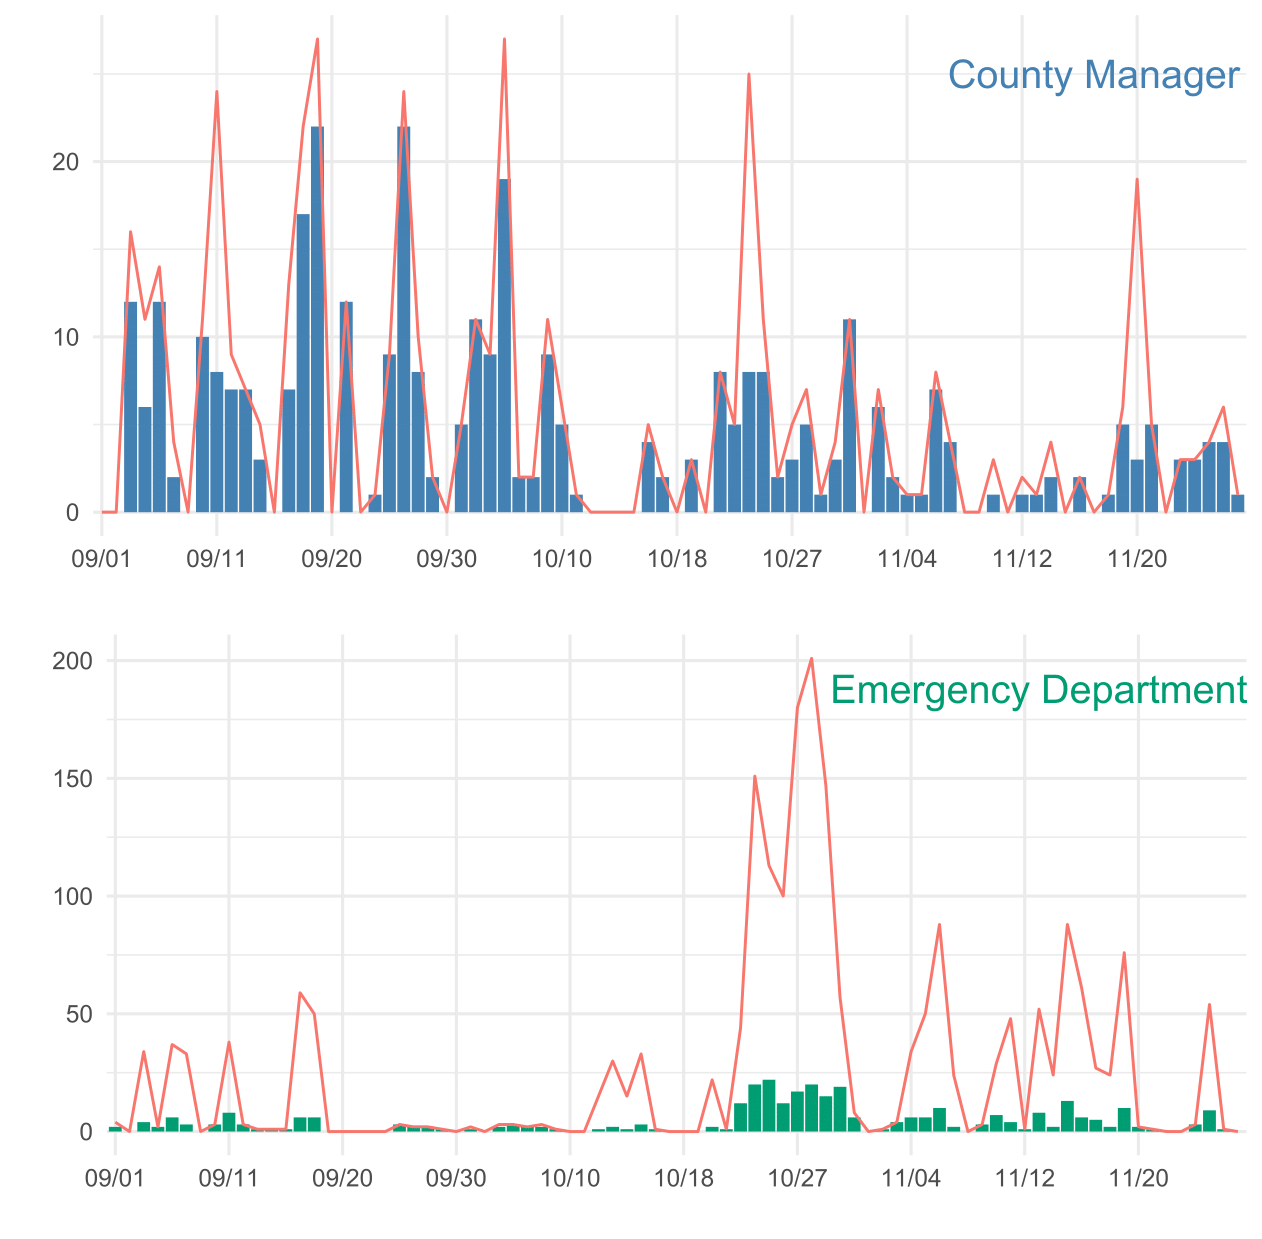
\includegraphics[width=.48\textwidth]{plots/EDAplot.png}  
	\caption{Sending behavior of two most active nodes in Dare County email data between 09/01/2012 and 11/30/2012. \textit{Top}: the number of emails per day sent by County manager (blue bar) and the number of recipients from this person per day (red line). \textit{Bottom}: the number of emails per day sent by emergency department official (green bar) and the number of recipients from this person per day (red line).}
\label{fig:EDAplot}
\vskip -0.15in
\end{figure}
\section{Interaction-partitioned Topic Model}\label{sec:model definition}

Data generated under the IPTM consists of $D$ unique documents. A single document, indexed by $d \in [D]$, is represented by the four components: the author $a_d \in [A]$, an indicator vector of recipients $\boldsymbol{r}_d = \{u_{dr} \}_{r=1}^{A}$, the timestamp $t_d \in (0, \infty)$, and a set of tokens $\boldsymbol{w}_d= \{w_{dn} \}_{n=1}^{N_d}$ that comprise the text of the document, where $N_d$ denotes the total number of tokens in a document. For simplicity, we assume that documents are ordered by time such that $t_d < t_{d+1}$.

\subsection{Interaction Patterns}\label{subsec:Interaction patterns}
They key idea that combines the IPTM component modeling ``what" with
the component modeling ``who," ``whom," and ``when" is that different
documents comes from the introduction of ``interaction patterns".  Each interaction pattern $c \in [C]$ is characterized by a set of dynamic network features---such as the number of messages sent from $a$ to $r$ in some time interval---and corresponding coefficients. We associate each document with the interaction pattern that best describes how people interact, and that is reflected to what people talk about via topic assignments. To be specific, we assume an interaction-pattern distribution over $C$ unique interaction patterns
\begin{equation}
	\boldsymbol{\psi}\sim \mbox{Dirichlet}\Big(\zeta, (\frac{1}{C},\ldots,\frac{1}{C})\Big),
\end{equation}
where $\zeta$ is the concentration parameter, and then each document $d \in [D]$ draws an interaction pattern $c_d$ as below:
\begin{equation}
c_d\sim \mbox{Multinomial}(\boldsymbol{\psi}).
\end{equation}


\subsection{Content Generating Process}\label{subsec:Content generating process}

The words $\boldsymbol{w}_d$ are generated according to the cluster-based topic model \cite{wallach2008structured}, an extension of a well-known Bayesian topic model, latent Dirichlet allocation (LDA) \cite{Blei2003}. As in LDA, we generate the corpus-wide global variables that describe the content via topics. First, we model each topic $k\in [K]$ as a discrete distribution over $V$ unique word types 
\begin{equation}
\boldsymbol{\phi}_k \sim \mbox{Dirichlet}\Big(\beta, (\frac{1}{V},\ldots,\frac{1}{V})\Big),
\end{equation}
where $\beta$ is the concentration parameter. Next, following the cluster-based topic model, document $d$ has the document-topic distribution
\begin{equation}
	\boldsymbol{\theta}_d \sim \mbox{Dirichlet}(\alpha, \boldsymbol{m}_{c_d}),
\end{equation}
where $\alpha$ are the concentration parameter and $\boldsymbol{m}=(m_1,\ldots,m_K)$ is the base measure.
In order to capture the overall prevalence of each topic in the corpus, we assume that each $\boldsymbol{m}_{c}$ is given Dirichlet priors with a single corpus-level base measure $\boldsymbol{m}$
	\begin{equation}
\boldsymbol{m}_c\sim \mbox{Dirichlet}\Big(\alpha_1, \boldsymbol{m}\Big),
	\end{equation}
	where $\alpha_1$ is the concentration parameter determining the extent to which the group-specific base measures are affected by the corpus-level base measure. Finally, the corpus-level base measure is assumed to have Dirichlet prior with uniform base measure
		\begin{equation}
			\boldsymbol{m}\sim \mbox{Dirichlet}\Big(\alpha_0, (\frac{1}{K},\ldots,\frac{1}{K})\Big).
		\end{equation}
	Given that $\bar N_d = \max(1, N_d)$ where $N_d$ is known, a topic $z_{dn}$ is drawn from the document-topic distribution and then a word $w_{dn}$ is drawn from the chosen topic for each $n \in [\bar N_d]$---i.e.,
\begin{equation}
\begin{aligned}
&z_{dn} \sim \mbox{Multinomial}(\boldsymbol{\theta}_d),\\
&w_{dn} \sim\mbox{Multinomial} (\phi_{z_{dn}}).
\end{aligned}
\end{equation}


\subsection{Tie Generating Process}\label{subsec:Tie generating process}
We generate ties---author $a_d$, recipients $\boldsymbol{r}_d$, and timestamp $t_d$---using a continuous-time process
that depends on the interaction patterns' various features. Conditioned on the document-specific interaction pattern (Seciton \ref{subsec:Interaction patterns}), we assume the following steps of tie generating process. Much like in the SAOM \cite{snijders2010introduction}, we conceptualize tie generation as a process that is governed by senders acting in continuous time. 

\subsubsection{Latent Recipients}\label{subsubsec:Hypothetical Recipients}
For every possible author--recipient pair $(a,r)_{a \neq r}$, we define the ``recipient intensity", which is the likelihood of document $d$ being sent from $a$ to $r$:
\begin{equation}
\lambda_{adr} = {\boldsymbol{b}_{c_d}}^{\top}\boldsymbol{x}_{adrc_d},
\end{equation}
where $\boldsymbol{b}_c$ is $P$--dimensional vector of coefficients and $\boldsymbol{x}_{adrc}$ is a set of network features which vary depending on the hypotheses regarding canonical processes relevant to network theory such as popularity, reciprocity, and transitivity. We place a Normal prior $\boldsymbol{b}_c \sim N(\boldsymbol{\mu}_b, \Sigma_b)$.

In the example of email networks, we form the covariate vector for recipients $\boldsymbol{x}_{adrc}$ using dynamic network statistics on three time intervals prior to $t^+_{d-1}$ (i.e., immediately after the previous document was sent). We compute eight network statistics within each time interval \cite{PerryWolfe2012}, where the intervals are $[t^+_{d-1}-384h, t^+_{d-1}-96h), [t^+_{d-1}-96h, t^+_{d-1}-24h)$ and $[t^+_{d-1}-24h, t^+_{d-1})$. We define the intervals to have equal length in the log-scale, and use $i=1$ to denote the earliest interval---i.e., $[t^+_{d-1}-384h, t^+_{d-1}-96h)$---and i = 3 to denote the latest. The network statistics (illustrated in Figure \ref{fig:dynamic network statistics}) are:
\begin{figure}[b]
	\vskip -0.1in
	\centering
	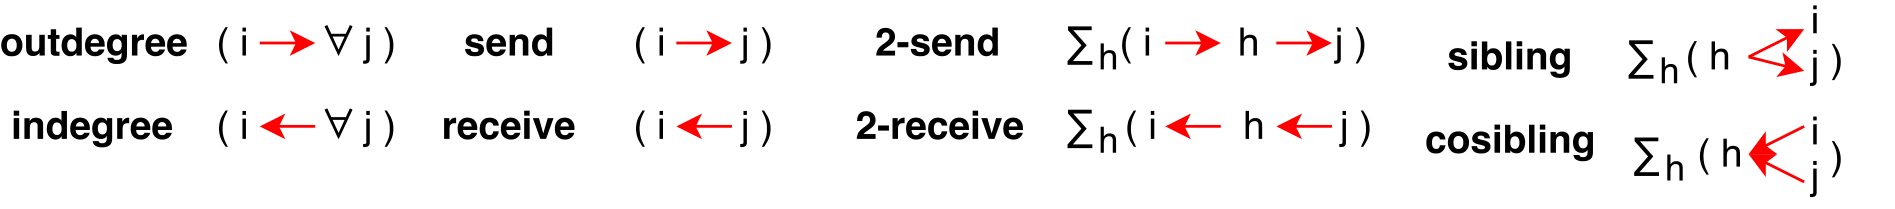
\includegraphics[height= 1.5cm, trim= 0cm 0cm 37cm 0cm, clip=true]{plots/netstats-1.png} \vspace{-.1cm}
	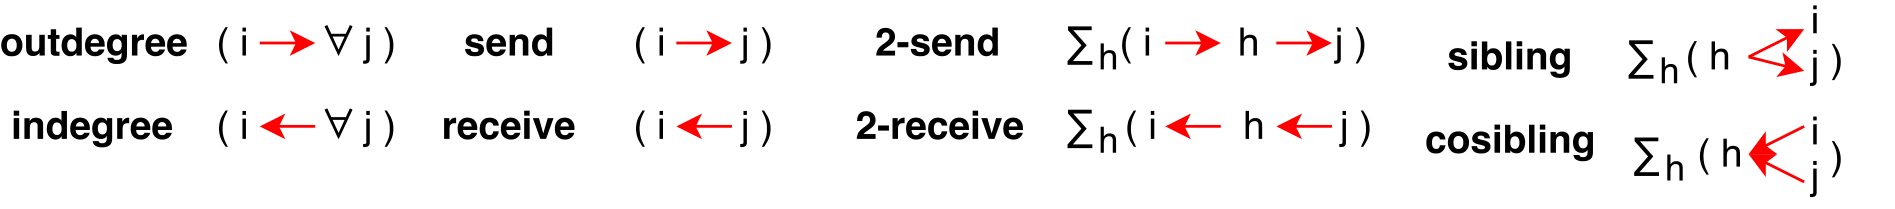
\includegraphics[height=1.5cm,, trim= 30cm 0cm 0cm 0cm, clip=true]{plots/netstats-1.png}
	\caption{Eight dynamic network statistics used for the application to email networks.}
	\label{fig:dynamic network statistics}	
\end{figure}
\begin{itemize}
	\item[1.] outdegree$(a,c,i)=\sum\limits_{d^\prime:t_{d^\prime \in i}} I(c_{d^\prime} = c)I(a_{d^\prime} = a)$;
	\item[2.] indegree$(r,c,i)=\sum\limits_{d^\prime:t_{d^\prime \in i}} I(c_{d^\prime} = c)I(u_{d^\prime r} = 1)$;
	\item[3.] send$(a,r,c,i)$\\
	$=\sum\limits_{d^\prime:t_{d^\prime \in i}} I(c_{d^\prime} = c)I(a_{d^\prime} = a)I(u_{d^\prime r} = 1)$;
	\item[4.] receive$(a,r,c,i)=\mbox{send}(r,a,c,i)$;
	\item[5.] 2-send$(a,r,c,i) $\\= $\sum\limits_{\substack{i^\prime, i^{\prime\prime}\geq i:\\i^\prime = i \mbox{ \small or }i^{\prime\prime}=i}}\sum\limits_{h \neq a, r} \mbox{send}(a,h,c,i^\prime)\mbox{send}(h,r,c,i^{\prime\prime})$;
	\item[6.] 2-receive$(a,r,c,i) $\\= $\sum\limits_{\substack{i^\prime, i^{\prime\prime}\geq i:\\i^\prime = i \mbox{ \small or }i^{\prime\prime}=i}}\sum\limits_{h \neq a, r} \mbox{send}(h,a,c,i^\prime)\mbox{send}(r,h,c,i^{\prime\prime})$;
	\item[6.] sibling$(a,r,c,i) $\\= $\sum\limits_{\substack{i^\prime, i^{\prime\prime}\geq i:\\i^\prime = i \mbox{ \small or }i^{\prime\prime}=i}}\sum\limits_{h \neq a, r} \mbox{send}(h,a,c,i^\prime)\mbox{send}(h,r,c,i^{\prime\prime})$;
	\item[6.] cosibling$(a,r,c,i) $\\= $\sum\limits_{\substack{i^\prime, i^{\prime\prime}\geq i:\\i^\prime = i \mbox{ \small or }i^{\prime\prime}=i}}\sum\limits_{h \neq a, r} \mbox{send}(a,h,c,i^\prime)\mbox{send}(r,h,c,i^{\prime\prime})$;
\end{itemize}
where $I(\cdot)$ is an indicator function. Note that in order to obtain two-path statistics (i.e., 2-send, 2-receive, sibling, and cosibling) within a single time interval $i$, we compute the number of two-paths from $a$ to $r$ in interaction pattern $c$ by summing over the pairs of intervals $(i^\prime, i^{\prime\prime})$ where the earlier email in the path was sent during interval $i$. 

Next, we hypothesize ``If $a$ were the
author of document $d$, who would be the recipent/recipients?" To do this, we draw each author's set of recipients from a non-empty Gibbs measure \cite{fellows2017removing}---a probability measure we defined in order to 1) allow multiple recipients or ``multicast", 2) prevent from obtaining zero recipient, and 3) ensure tractable normalizing constant. 

Because the IPTM allows multicast, we draw a binary (0/1) vector $\boldsymbol{u}_{ad}= (u_{ad1},
\ldots, u_{adA})$
\begin{equation} \boldsymbol{u}_{ad}  \sim
\mbox{Gibbs}(\delta, \boldsymbol{\lambda}_{ad}),
\end{equation}
where $\delta$ is a real number controlling the average number of recipients and $\boldsymbol{\lambda}_{id}= \{\lambda_{adr}\}_{r=1}^A$. We place a Normal prior $\delta \sim N(\mu_\delta,\sigma^2_\delta)$. In particular, we define $\mbox{Gibbs}(\delta, \boldsymbol{\lambda}_{ad})$ as
\begin{equation}
\begin{aligned}
&p(\boldsymbol{u}_{ad}|\delta, \boldsymbol{\lambda}_{ad}) \\&= \frac{\exp\Big\{\mbox{log}\big(\text{I}( \lVert \boldsymbol{u}_{ad}\rVert_1 > 0 )\big) + \sum_{r\neq a} (\delta+\lambda_{adr})u_{adr}\Big\}}{Z(\delta,\boldsymbol{\lambda}_{ad})} ,
\end{aligned}
\label{eqn:Gibbs}
\end{equation}
where $Z(\delta,\boldsymbol{\lambda}_{ad})= \prod_{r \neq a} (\mbox{exp}\{\delta+\lambda_{adr}\} + 1)-1$ is the normalizing constant and $\lVert \cdot \rVert_1$ is the $l_1$--norm. We provide the derivation of the normalizing constant as a tractable form in the supplementary material. 

\subsubsection{Latent Timestamps}\label{subsubsec:Hypothetical Timestamps}
Similarly, we hypothesize ``If $a$ were the author of document $d$, when would it be sent?" and define the ``timing rate" for author $i$
\begin{equation}
\mu_{ad} = g^{-1}(\boldsymbol{\eta}_{c_d}^\top \boldsymbol{y}_{adc_d}),
\end{equation}
where $\boldsymbol{\eta}_c$ is $Q$--dimensional vector of coefficients with a Normal prior $\boldsymbol{\eta}_c \sim N(\boldsymbol{\mu}_\eta,\Sigma_\eta)$, $\boldsymbol{y}_{adc}$ is a set of time-related covariates, which can be any feature that could affect timestamps of the document, and $g(\cdot)$ is the appropriate link function such as identity, log, or inverse. 

For example, the covariate vector for timestamps $\boldsymbol{y}_{adc}$ can include author-specific intercepts to account for individual differences in document-sending behavior. In addition, temporal features which possibly affect ``when to send" can be added---e.g., an indicator of weekends/weekdays and an indicator of AM/PM when the previous document was sent. 

In modeling ``when", we do not directly model the timestamp $t_d$. Instead, we assume that each author's the time-increment or ``time to next document" (i.e., $\tau_{d} = t_d-t_{d-1}$) is drawn from a specific distribution in the exponential family.  We follow the generalized linear model framework:
\begin{equation}
\begin{aligned}
E(\tau_{ad}) &= \mu_{ad},\\
V(\tau_{ad}) &= V(\mu_{ad}),
\end{aligned}
\end{equation}
where $\tau_{ad}$ is a positive real number. Possible choices of distribution include Exponential, Weibull, Gamma, and lognormal\footnote{lognormal distribution is not exponential family but can be used via modeling of $\log(\tau_d)$.} distributions, which are commonly used in time-to-event modeling. Based on the choice of distribution, we may introduce any additional parameter (e.g., $\sigma_\tau^2$) to account for the variance.

Our preliminary analysis revealed that the Dare County email networks and the Enron data set showed the best fitting when we assume lognormal distribution on the observed time-increments---i.e., $\log(\tau_{a_dd}) \sim N(\mu_{a_d d}, \sigma^2_\tau)$---compared to Gamma or Weibull distributions. We also observed significant lack-of-fit for single parameter distribution (e.g., Exponential distribution) since it failed to capture the variance in time-increments. Therefore, we chose lognormal distribution by taking the log-transformation and apply $\mu = E(\log(\tau_{ad})) = \mu_{ad}$ and $ \sigma_\tau^2=V(\log(\tau_{ad})) = V(\mu_{ad})$, using identity link function $g = I$. 
\subsubsection{Actual Data}\label{subsubsec:Actual Data}
Finally, we choose the actual author, recipients, and timestamp---which will be observed---by selecting the author--recipient-set pair with the smallest time-increment \cite{snijders1996stochastic}:
\begin{equation}
\begin{aligned}
a_d &= \mbox{argmin}_{a}(\tau_{ad}),\\
\boldsymbol{r}_d &= \boldsymbol{u}_{a_d d},\\
t_d &=t_{d-1} + \tau_{a_d d}.
\end{aligned}
\end{equation}
Therefore, it is an author-driven process in that the author of a document determines its recipients and its timestamp, based on the author's urgency to send the document to chosen recipients. 

\section{Posterior Inference}\label{sec:Inference}
Given that we only observe the authors, recipients, timestamps, and tokens $ \{ (a_d, \boldsymbol{r}_d, t_d,  \boldsymbol{w}_d)\}_{d=1}^D$ in real-world, our inference goal is to invert the generative process to obtain the posterior distribution over the unknown parameters, conditioned on the observed data and hyperparamters $\alpha_0, \alpha_1, \alpha, \beta, \zeta, \boldsymbol{\mu}_b, \Sigma_b, \boldsymbol{\mu}_\eta, \Sigma_\eta, {\mu}_\delta,\sigma^2_\delta$. After integrating out $\Phi$, $\Psi$, and $\Theta$ using Dirichlet-multinomial conjugacy \cite{griffiths2004finding}, we draw the samples using Markov chain Monte Carlo (MCMC) methods, repeatedly resampling the value of each parameter from its conditional posterior given the observed data, hyperparamters, and the current values of the other parameters. We express each parameter’s conditional posterior in a closed form using the data augmentation schemes in $\boldsymbol{u}$ \cite{tanner1987calculation}. In this section, we outline a Metropolis-within-Gibbs sampling algorithm and each latent variable's conditional posterior. Pseudocode is provided in the supplementary material.

First, since $u_{adr}$ is a binary random variable, new values may be sampled directly using
\begin{equation}
\begin{aligned}
&P(u_{adr}=1| \boldsymbol{u}_{ad\backslash r}, \boldsymbol{c},\boldsymbol{b}, \delta, \boldsymbol{x})
\propto \mbox{exp}\{\delta+\lambda_{adr}\};\\
&P(u_{adr}=0| \boldsymbol{u}_{ad\backslash r}, \boldsymbol{c},\boldsymbol{b}, \delta, \boldsymbol{x})\propto \text{I}(\lVert\boldsymbol{u}_{ad\backslash r}\rVert_1 > 0 ),
\end{aligned}
\label{eqn:latentreceiver}
\end{equation}
where $I(\cdot)$ is the indicator function that is used to prevent from the instances where the author has no recipients to send the document.

Next, the conditional posterior for topic assignment $z_{dn}$ is derived by multiplying the two sampling equations of the cluster-based topic model:
\begin{equation}
	\begin{aligned}
		&p(z_{dn}=k| \boldsymbol{z}_{\backslash dn}, \boldsymbol{c}, \boldsymbol{w}, \alpha_0, \alpha, \beta)\\
		%&\propto P(z_{dn}=k| \boldsymbol{z}_{\backslash dn}, c_d, \alpha_0, \alpha)\times P(w_{dn}|z_{dn}=k, \boldsymbol{z}_{\backslash dn}, \boldsymbol{w}, \beta)\\
		&\propto 
		\Big(\hat N_{dk, \backslash dn}+\alpha \frac{\hat N_{kc_d,\backslash dn}+\alpha_1\frac{\hat N_{k, \backslash dn}+\frac{\alpha_0}{K}}{\hat N_{\backslash dn}+\alpha_0}}{\hat N_{c_d, \backslash dn}+\alpha_1}	\Big)\\&\quad\quad\times \Big(\frac{\hat N_{w_{dn}k, \backslash dn}+\frac{\beta}{V}}{\hat N_{k, \backslash dn}+\beta}	\Big),
	\end{aligned}
\end{equation}
where $\hat N$ are defined according to the minimal path assumption \cite{wallach2008structured}.
Specifically, $\hat N_{dk, \backslash dn}$ is the number of times topic $k$ has been used in document $d$, $\hat N_{kc_d, \backslash dn}$ is the number of different documents belonging to $c_d$ that use topic $k$, $\hat N_{k, \backslash dn}$ is the number of different interaction patterns in which $k$ has been used, $\hat N_{w_{dn}k, \backslash dn}$ is the number of tokens assigned to topic $k$ whose type is the same as that of $w_{dn}$, and the subscript $\backslash dn$ denotes the exclusion of $n^{th}$ element in document $d$. 

For each document $d \in [D]$, we sample interaction-pattern assignment from the discrete distribution over $C$ interaction patterns using 
\begin{equation}
\begin{aligned}
&P(c_d = c|\boldsymbol{z}, \zeta, \boldsymbol{u},\boldsymbol{a}, \boldsymbol{t})
\\&\propto P(c_d=c|\boldsymbol{c}_{\backslash d}, \zeta) P(\boldsymbol{z}_d|\gamma, \alpha, c_d=c, \boldsymbol{c}_{\backslash d}, \boldsymbol{z}_{\backslash d})\\&\times P(a_d, t_d|c_d = c, \boldsymbol{\eta}, \sigma_\tau^2) P(\boldsymbol{u}|c_d=c, \boldsymbol{c}_{\backslash d}, \boldsymbol{b}, \delta) 
\\&\propto (\hat N_{c, \backslash d}+\frac{\zeta}{C}) \\&
\times\prod_{n=1}^{\bar N_d} (\hat N_{dz_{dn}, \backslash dn}+\alpha \frac{\hat N_{z_{dn}c,\backslash dn}+\alpha_1\frac{\hat N_{z_{dn}, \backslash dn}+\frac{\alpha_0}{K}}{\hat N_{\backslash dn}+\alpha_0}}{\hat N_{c, \backslash dn}+\alpha_1})\\&\times
\varphi_{\tau}(\tau_{d}; \mu_{a_d d}, \sigma_\tau^2)\times \prod_{a\neq a_d}\big(1-\Phi_{\tau}(\tau_{d}; \mu_{a d}, \sigma_\tau^2) \big)\\& 
\times
\prod_{a=1}^A \frac{\exp\Big\{\mbox{log}\big(\text{I}( \lVert \boldsymbol{u}_{ad}\rVert_1 > 0)\big) + \sum\limits_{r \neq a} (\delta+\lambda_{adr})u_{adr}\Big\}}{Z(\delta,\boldsymbol{\lambda}_{ad})}.
\end{aligned}
\end{equation}

New values for continuous variables $\delta, \boldsymbol{b},$ and $\boldsymbol{\eta}$ and $\sigma^2_\tau$ (if applicable) cannot be sampled directly from their conditional posteriors, but may instead be obtained using the Metropolis--Hastings algorithm. With uninformative priors (i.e., $N({0},\infty)$), the conditional posterior over $\delta$ and $\boldsymbol{b}$ is
\begin{equation}
 	   \prod_{d=1}^D
 	   \prod_{a=1}^A \frac{\exp\Big\{\mbox{log}\big(\text{I}( \lVert \boldsymbol{u}_{ad}\rVert_1 > 0)\big) + \sum\limits_{r \neq a} (\delta+\lambda_{adr})u_{adr}\Big\}}{Z(\delta,\boldsymbol{\lambda}_{ad})},
 	   \end{equation}
 	   where the two variables share the conditional posterior and thus can be jointly sampled. Likewise, assuming uninformative priors on $\boldsymbol{\eta}$ (i.e., $N({0},\infty)$) and $\sigma_{\tau}^2$ (i.e., half-Cauchy($\infty$)), the conditional posterior is
 	   \begin{equation}
 	   \prod_{d=1}^D\Big(\varphi_{\tau}(\tau_{d}; \mu_{a_d d}, \sigma_\tau^2)\times \prod_{a\neq a_d}\big(1-\Phi_{\tau}(\tau_{d}; \mu_{a d}, \sigma_\tau^2) \big)\Big).
 	   \end{equation}
 	   
 	   Although the IPTM is a highly complex model with a lot of latent variables, it yields an efficient inference algorithm by taking advantage of the two main parts of the likelihood  repeatedly appear in the sampling equations---one from the latent recipients (Section \ref{subsubsec:Hypothetical Recipients}) and another from the latent timestamps (Section \ref{subsubsec:Hypothetical Timestamps}). %In addition, for better performance and interpretability of the topics we infer, we adopt the hyperparameter optimization technique for $\alpha$ and $\boldsymbol{m}$ called ``new fixed-point iterations using the Digamma recurrence relation'' in \cite{wallach2008structured}, for every outer iteration. 
 	   
 	   \section{Data}\label{sec:Data}
 	   Our data come from the North Carolina county government email dataset collected by \cite{ben2017transparency} that includes internal email corpora covering the inboxes and outboxes of managerial-level employees of North Carolina county governments. Out of over twenty counties, we chose Dare County to 1) see whether and how communication networks surrounding a notable national emergency---Hurricane Sandy---differed from those surrounding other governmental functions, and 2) limit the scope of this initial application. The Dare County email network contains 2,247 emails, sent and received by 27 department managers over a period of 3 months (September--November) in 2012. 
 	   
 	   To verify that our model is applicable beyond the Dare County email network, we also performed two validation experiments using the Enron data set \cite{klimt2004introducing}. We took a subset of the original data such that we only include emails between actors who sent over 300 emails, and actors who received over 300 emails from the chosen authors. Emails that were not sent to at least one other active actor were discarded, which resulted in a total of 6,613 emails involving 30 actors. For the Enron data set, we changed the time unit from hour to day in modeling the timestamps.
 	   
 	   \section{Experiments}\label{sec:Experiments}
 	   We conducted a set of posterior predictive experiments---1) out-of-sample tie predictions, 2) topic coherence, and 3) posterior predictive checks---to gauge the IPTM's predictive performance as compared to alternative modeling approaches.
 	   
 	   \subsection{Out-of-Sample Tie Predictions}\label{subsec:Tie Prediction}
 	   We evaluated the IPTM's ability to predict ties in textual communications from either the Dare County email network or the Enron data set, conditioned on the text of those emails and ``training" part of the data. We separately formed a test split of each three components---author, recipients, and timestamps---by randomly selecting ``test" data with probability $p=0.1$. Any missing variables were imputed by drawing samples from their conditional posterior distributions, given the observed data, estimates of latent variables, and current estimates of test data. The full conditional posterior distributions for ``test" author, recipients, and timestamps are provided in the supplementary material.
 	   
 	   We then run inference to update the latent variables given the imputed and observed data. We iterate the two steps---imputation and inference---multiple times to obtain enough number of estimates for ``test" data. Algorithm \ref{alg:PPE} outlines this procedure.
 	   
 	   \begin{algorithm}[H]
 	   	\caption{Out-of-Sample Tie Predictions}
 	   	\label{alg:PPE}
 	   	\begin{algorithmic}
 	   		\STATE {\bfseries Input:} data $ \{ (a_d, \boldsymbol{r}_d, t_d,  \boldsymbol{w}_d)\}_{d=1}^D$, \\
 	   		number of new data to generate $R$,\\
 	   		number of interaction patterns and topics $(C, K)$,\\
 	   		hyperparameters $(\alpha_0, \alpha_1, \alpha, \beta, \zeta, \boldsymbol{\mu}_b, \Sigma_b, \boldsymbol{\mu}_\eta, \Sigma_\eta, {\mu}_\delta,\sigma^2_\delta)$\\
 	   		\vskip 0.1in
 	   		\textbf{Test splits:}	
 	   		\STATE Draw test authors with $p=0.1$ (out of $D$ authors) 
 	   		\STATE Draw test elements of recipient vector 
 	   		with $p=0.1$ (out of $D\times (A-1)$ receipient indicators $\{\{\boldsymbol{r}_{dr}\}_{r\in [A]_{\backslash a_d}}\}_{d=1}^D$)
 	   		\STATE Draw test timestamps with $p=0.1$  (out of $D$ timestamps) 
 	   		\STATE Set the ``test" data as ``missing" (NA)
 	   		\vskip 0.1in
 	   		\textbf{Imputation and inference:}	
 	   		\STATE Initialize the parameters $(\boldsymbol{l}, \boldsymbol{z}, \boldsymbol{b}, \boldsymbol{\eta},\delta, \boldsymbol{u})$
 	   		\FOR{$r=1$ {\bfseries to}  $R$}
 	   		\FOR{$d=1$ {\bfseries to}  $D$}
 	   		\IF{$a_d=$  NA}
 	   		\FOR{$a=1$ {\bfseries to} $A$}
 	   		\STATE Compute $\pi_{a} $ using $P(a_d= a | \cdot)$
 	   		\ENDFOR
 	   		\STATE Draw $a_d \sim \mbox{Multinomial}(\pi)$
 	   		\ENDIF
 	   		\FOR{$r\in [A]_{\backslash a_d}$}
 	   		\IF{$r_{dr}=$ NA}
 	   		\STATE Draw $r_{dr}$ using $P(r_{dr}= 1 | \cdot)$ and $P(r_{dr}= 0| \cdot)$ 
 	   		\ENDIF
 	   		\ENDFOR
 	   		\IF{$t_d=$ NA}
 	   		\STATE Draw proposal $\boldsymbol{\tau}^{new}_d \sim \mbox{lognormal}(\mu_{a_dd}, \sigma^2_\tau)$
 	   		\STATE Use Metropolis-Hastings to decide accept or reject using the probability
 	   		    \begin{equation*}
 	   		    \footnotesize
\frac{P(\boldsymbol{\tau}^{new}_d|\mu_{a_dd}, \sigma^2_\tau) P(\boldsymbol{\tau}^{new}_d| \cdot)}{P(\boldsymbol{\tau}^{old}_d|\mu_{a_dd}, \sigma^2_\tau) P(\boldsymbol{\tau}^{old}_d| \cdot)},
 	   		    \end{equation*}
 	   		    where $\boldsymbol{\tau}^{old}_d$ is from earlier iteration.
 	   		\ENDIF
 	   		\STATE Run inference and update $(\boldsymbol{c}, \boldsymbol{z}, \boldsymbol{b}, \boldsymbol{\eta},\delta, \boldsymbol{u})$ given the imputed and observed data
 	   		\ENDFOR
 	   		\STATE Store the estimates for ``test" data
 	   		\ENDFOR
 	   	\end{algorithmic}
 	   \end{algorithm}
 	   
 	   We compared the IPTM's performance with that of baseline---the IPTM with $C=1$. This amounts to an ablation study \citep{richardson2006beyond,bilgic2010active}, as a single interaction pattern breaks the link between text and network structure in the IPTM. The text and network structure are linked through the assignment of topics to different interaction patterns, and with one interaction pattern all topics are associated with the same network structure. We do not define any other baselines (i.e., other models`test" a fr machine learning literature) to which to compare the predictive performance of the IPTM. We omit comparison to baselines because we are unable to identify existing models that can predict the same form of social data that can be modeled by the IPTM---a form that includes one out of $n$ authors, one through $n-1$ recipients, and a continuous and positive time point. Consider the prediction of e-mail recipients. As far as we are aware, the Gibbs measure model we derive is unique among existing methods in its ability to predict a set of one through $n-1$ (out of $n-1$) recipients of an e-mail. This is just the recipient component of the model---we are also not able to identify any other method that permits the prediction of the author, recipient multicast, and timing of ties. We could construct baseline models to compare in terms of predictive performance for each component of the social data (e.g., a regression model to predict e-mail timing, a multi-class classifier to predict author). However, that would be an arbitrary exercise, as it is not clear why we would select any particular baseline out of the dozens of candidates for each component of the social data modeled in the IPTM. 
 	   
 	   We varied the number of interaction patterns $C$ from 1 to 3 and the number of topics $K$ from 1 to 50 (Dare) or 100 (Enron) as a grid-search based hyperparameter selection process.  For each combinations of $C$ and $K$, predicted values of tie data were then compared to the true values to yield: $F_1$ scores for author predictions, multiclass version of the area under the ROC curve (AUC) measure \cite{hand2001simple} for reciptient predictions, and median absolute error (MAE) on timestamp predictions. We show the tie prediction results, averaged over five random test splits of each tie component, in Figure \ref{fig:PPE} \textcolor{red}{(Plots to be updated)}. Although our model is intended for exploratory analysis, it achieves better link prediction performance than the baseline, validating our assumption that the IPTM acheives better predictive performance when topic-based contents are accounted to infer the parameters that govern the generation of tie data---authors, recipients, and timestamps.
 	   \begin{figure}[tb]
 	   	\centering
 	   	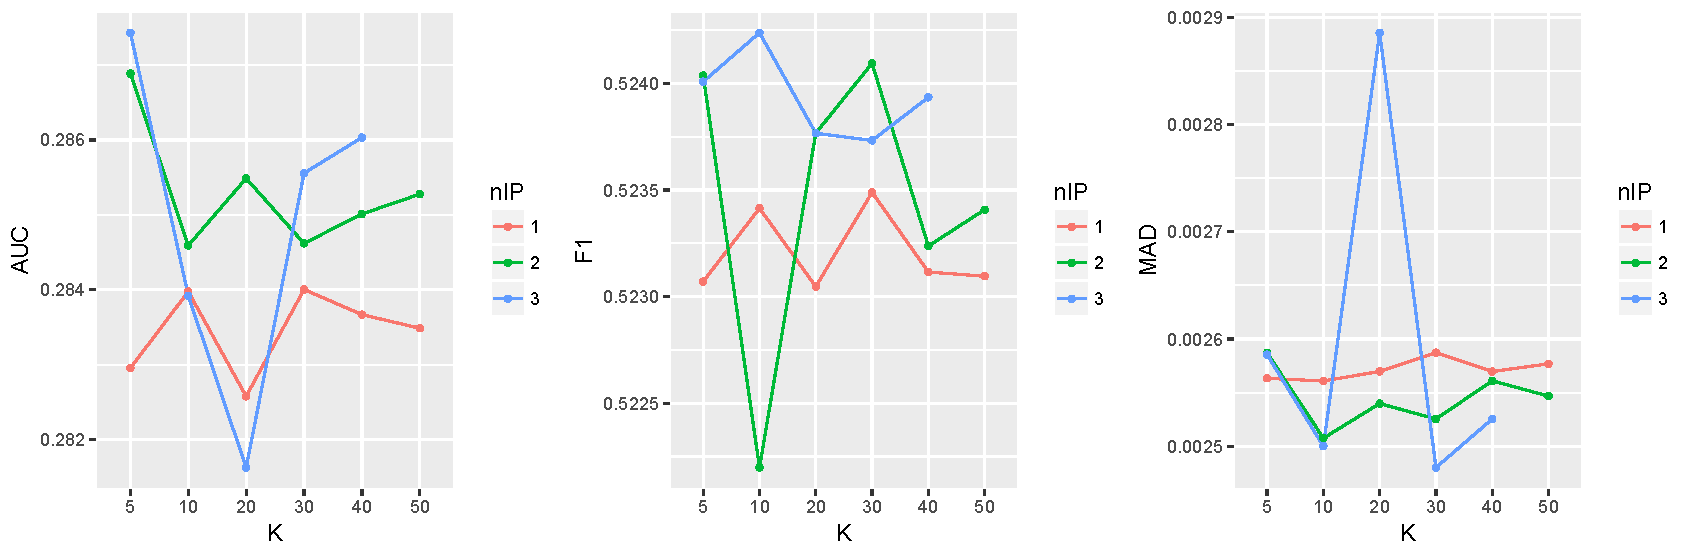
\includegraphics[width = 0.49\textwidth, trim= 0.7cm 0cm 0cm 0cm, clip=true]{plots/Dare_PPE.pdf} 
 	   	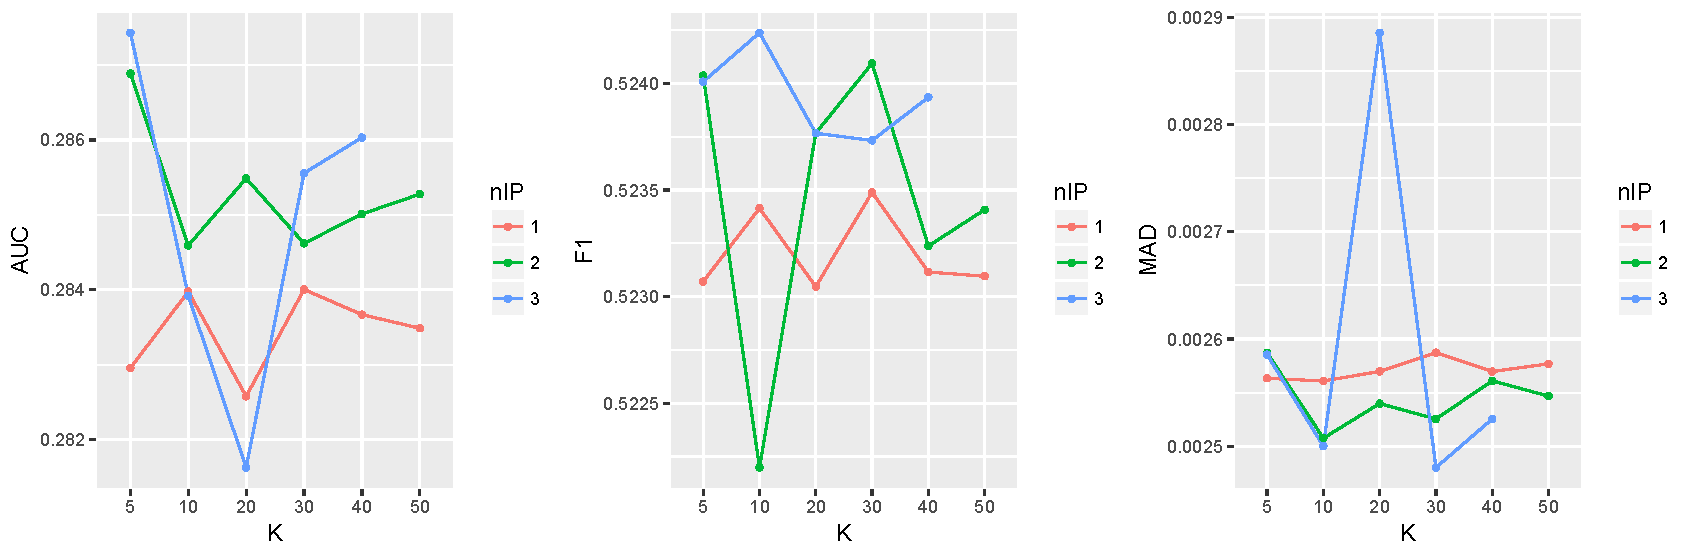
\includegraphics[width = 0.49\textwidth, trim= 0.7cm 0cm 0cm 0cm, clip=true]{plots/Dare_PPE.pdf}   
 	   	\caption{Average F1 score,  AUC, MAE of out-of-sample tie predictions. \textit{Top}: Dare County email network. \textit{Bottom}: the Enron dataset.}
 	   	\label{fig:PPE}	
 	   \end{figure}
 	   \subsection{Topic Coherence}\label{subsec:Topic Coherence}
 	   Topic coherence metrics \cite{mimno2011optimizing} are often used to evaluate the semantic coherence in topic models.To demonstrate that the IPTM's incorporation of network features improves the ability of modeling text, we compared the coherence of topics inferred using our model with the coherence of topics inferred using LDA. Instead of re-fitting the data using standard LDA algorithms, we used the topic assignments from the IPTM with $C=1$, which reduces the IPTM to LDA in terms of topic assignments. We varied the number of interaction patterns and the number of topics as in Section \ref{subsec:Tie Prediction}, and drew five samples from the joint posterior distribution over the latent variables. We evaluated the topics resulting from each sample and averaged over the five samples, where the results are shown in Figure \ref{fig:topic}. Combined with the findings in Section \ref{subsec:Tie Prediction}, this result demonstrates that the IPTM can achieve good predictive performance while producing coherent topics. 
 	   \begin{figure}[h]
 	   	\centering
 	   	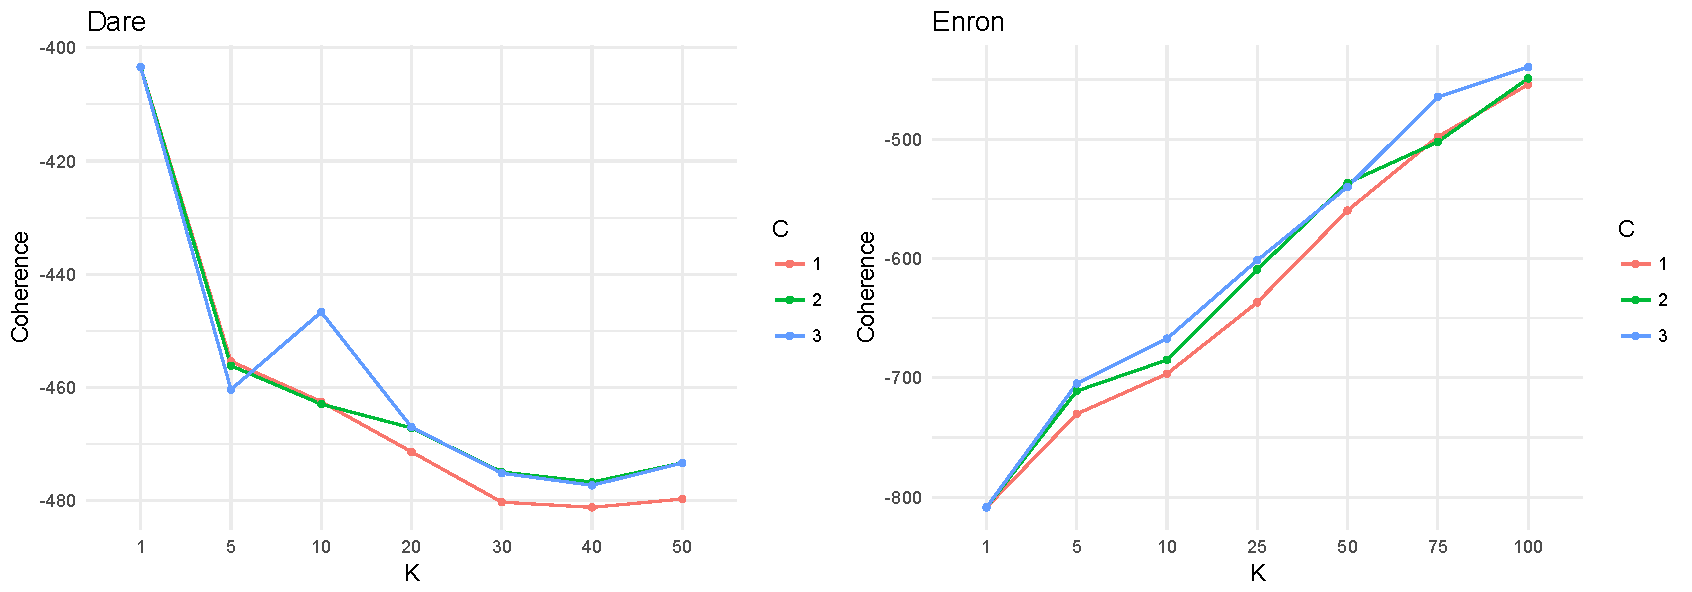
\includegraphics[width = 0.49\textwidth]{plots/topicplot.pdf}
 	   	\caption{Average topic coherence scores: (\textit{left}) Dare County email network. (\textit{right}) the Enron data set.}
 	   	\label{fig:topic}
 	   \end{figure}
 	   \subsection{Posterior Predictive Checks}\label{subsec:PPC}
 	   Finally, we performed posterior predictive checks \cite{rubin1984bayesianly} to evaluate the appropriateness of the model specification for the Dare County email network. We formally generated entirely new data, by simulating ties and contents $\{(a_{d}, \boldsymbol{r}_{d}, t_{d}, \boldsymbol{w}_{d})\}_{d=1}^D$ from the genenerative process in Section \ref{sec:model definition}, conditional upon a set of inferred parameter values from the inference in Section \ref{sec:Inference}. Pseudocode is provided in the supplementary material. We specified the number of interaction patterns as $C=?$ and the number of topics as $K = ?$, which yielded the best performance in Section \ref{subsec:Tie Prediction}. For the test of goodness-of-fit in terms of network dynamics, we defined multiple network statistics that summarize meaningful aspects of the Dare County email network: indegree distribution for author activities, outdegree distribution for recipient activities, recipient size distribution, document time-increments distribution, the edgewise shared partner distribution, and the geodesic distance distribution. We then generated 100 synthetic networks and texts from the posterior predictive distribution implied by the IPTM and Dare County email network.
 	   We applied each discrepancy function to each synthetic network to yield the distributions over the values of the six network statistics
 	   
 	   As shown in Figure \ref{fig:PPC} \textcolor{red}{(Plots to be updated)}, the IPTM shows ``good fit" for the Dare County email network in that the observed data is not an outlier with respect to the distributions of new data drawn from the posterior predictive distribution. The IPTM generated synthetic networks with indegree distribution, outdegree distribution, recipient size, document time-increments, and edgewise shared partners that are very similar to those of the Dare County email network, showing that the model captures some important work features of the data including spreadness and transitivity. 
 	   \begin{figure}[tb]
 	   	\centering
 	   	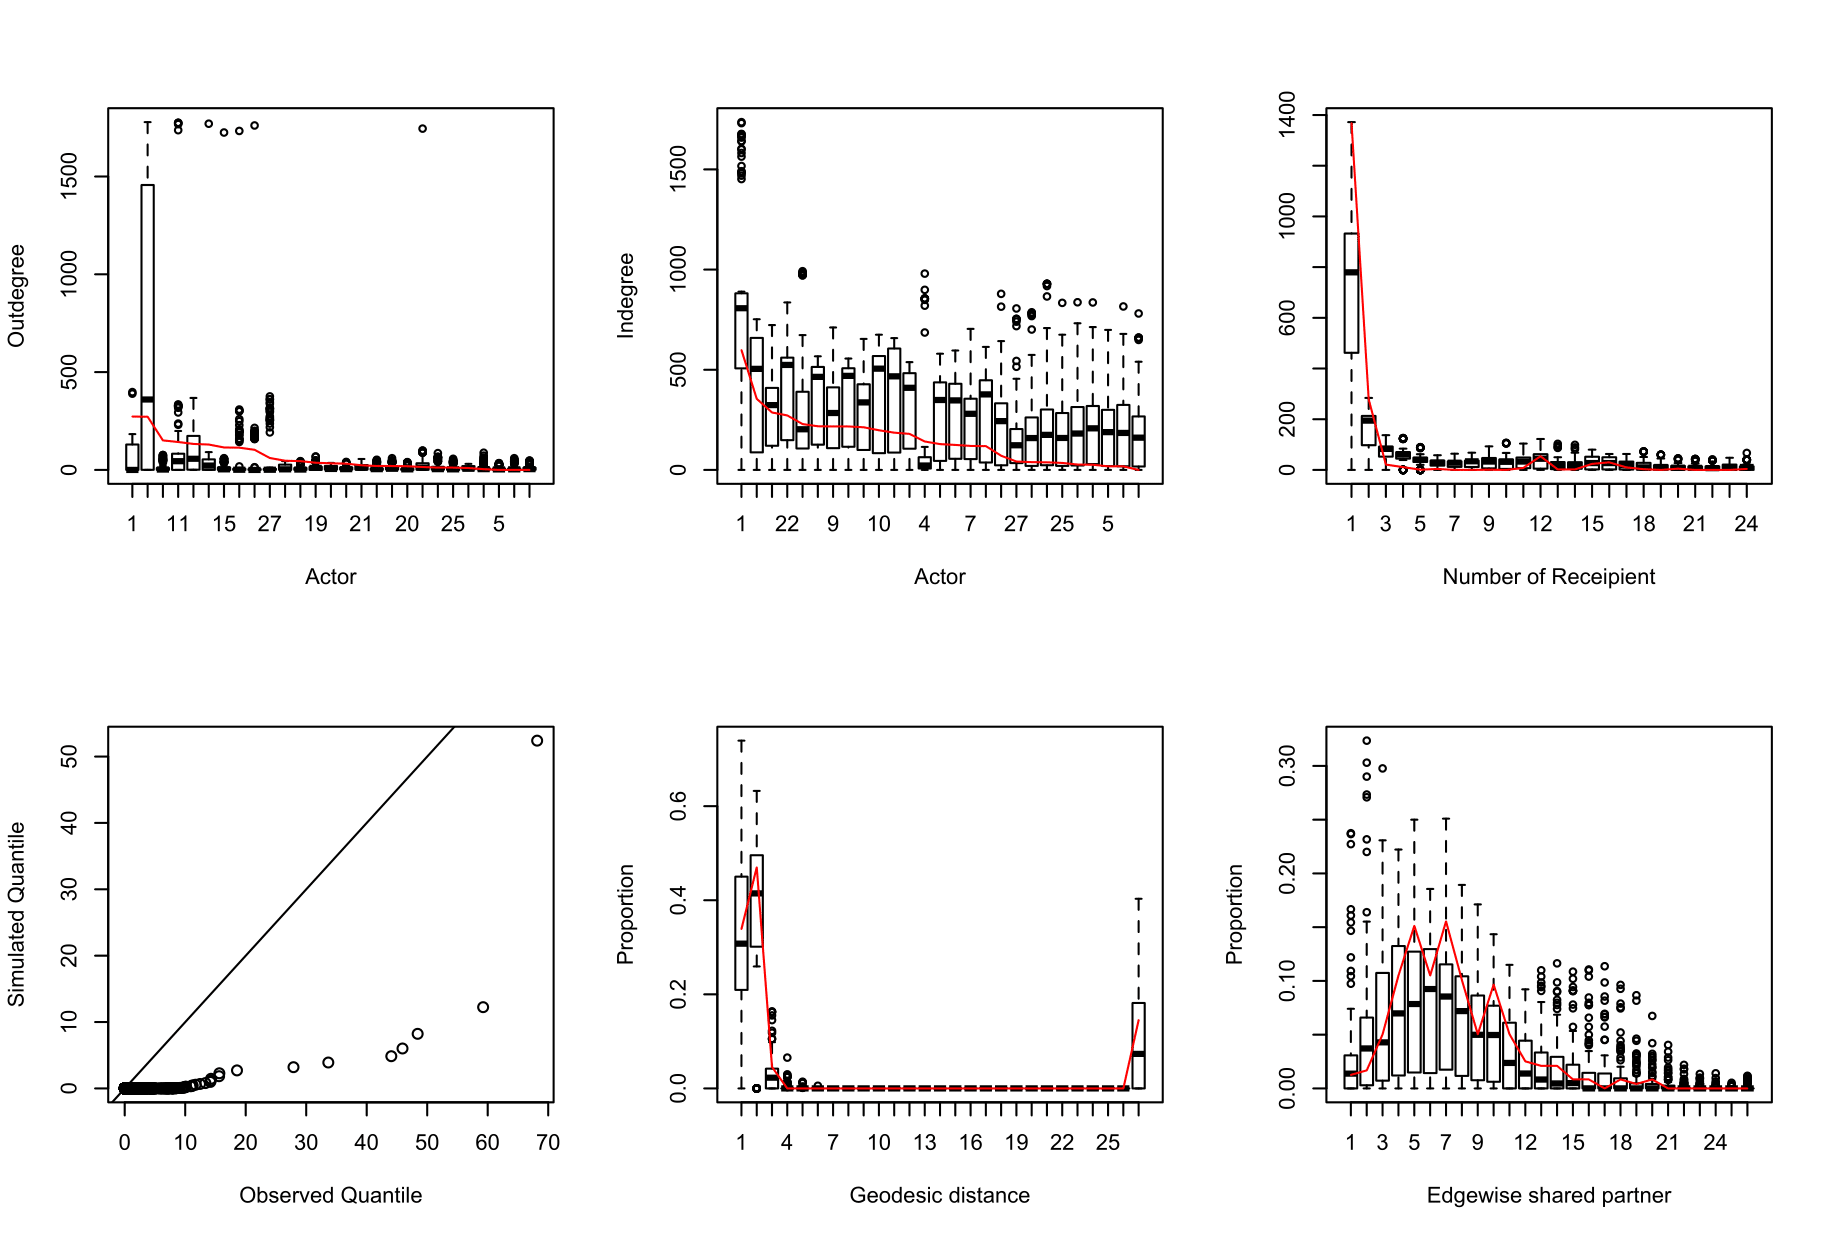
\includegraphics[width = 0.47\textwidth]{plots/PPC_plot-1.png}
 	   	\caption{Posterior predictive checks for the Dare County email network: (a) outdegree, (b) indegree, (c) recipient size, (d) QQplot of time-increments, (e) geodesic distance, and (f) edgewise shared partners.}
 	   	\label{fig:PPC}
 	   \end{figure}
 	   \section{Exploratory Analysis}\label{sec:Analysis}
 	   Our model is primarily intended as an exploratory analysis tool for time-stamped textual communication. Our main goal in this exploratory analysis was to test three hypotheses: 1) personal or social topics (if any) would exhibit strong reciprocity and transitivity in tie formation, 2) topics about dissemination of information would be characterized by a lack of reciprocity, and 3) topics about Hurricane Sandy would exhibit a very different
 	   interaction pattern from the normal day-to-day conversations.
 	   \subsection{Topic Assignments}\label{subsec:Topic Assignments}
 	   \subsection{Interaction Pattern Coefficients}\label{subsec:Interaction Pattern Coefficients}
 	   \section{Summary}\label{sec:Conclusions}
 	   The IPTM is, to our knowledge, the first model to be capable of jointly modeling the author, recipients, timestamps and contents in time stamped text-valued networks. The IPTM incorporates innovative components, including the modeling of multicast tie formation and the conditioning of ERGM style network generative features on topic-based content. The application to North Carolina county government email data demonstrates, among other capabilities, the effectiveness at the IPTM in separating out both the content and relational structure underlying the normal day-to-day function of an organization and the management of a highly time-sensitive event---Hurricane Sandy. Finally, although we presented the IPTM in the context of email networks, the IPTM is applicable to a variety of networks in which ties are attributed with textual documents. These include, for example, economic sanctions sent between countries and legislation attributed with sponsors and co-sponsors. 
% Acknowledgements should only appear in the accepted version.

% In the unusual situation where you want a paper to appear in the
% references without citing it in the main text, use \nocite
\nocite{langley00}

\bibliography{IPTM}
\bibliographystyle{icml2018}
%%%%%%%%%%%%%%%%%%%%%%%%%%%%%%%%%%%%%%%%%%%%%%%%%%%%%%%%%%%%%%%%%%%%%%%%%%%%%%%
%%%%%%%%%%%%%%%%%%%%%%%%%%%%%%%%%%%%%%%%%%%%%%%%%%%%%%%%%%%%%%%%%%%%%%%%%%%%%%%
% DELETE THIS PART. DO NOT PLACE CONTENT AFTER THE REFERENCES!
%%%%%%%%%%%%%%%%%%%%%%%%%%%%%%%%%%%%%%%%%%%%%%%%%%%%%%%%%%%%%%%%%%%%%%%%%%%%%%%
%%%%%%%%%%%%%%%%%%%%%%%%%%%%%%%%%%%%%%%%%%%%%%%%%%%%%%%%%%%%%%%%%%%%%%%%%%%%%%%
%%%%%%%%%%%%%%%%%%%%%%%%%%%%%%%%%%%%%%%%%%%%%%%%%%%%%%%%%%%%%%%%%%%%%%%%%%%%%%%
%%%%%%%%%%%%%%%%%%%%%%%%%%%%%%%%%%%%%%%%%%%%%%%%%%%%%%%%%%%%%%%%%%%%%%%%%%%%%%%

\end{document}


% This document was modified from the file originally made available by
% Pat Langley and Andrea Danyluk for ICML-2K. This version was created
% by Iain Murray in 2018. It was modified from a version from Dan Roy in
% 2017, which was based on a version from Lise Getoor and Tobias
% Scheffer, which was slightly modified from the 2010 version by
% Thorsten Joachims & Johannes Fuernkranz, slightly modified from the
% 2009 version by Kiri Wagstaff and Sam Roweis's 2008 version, which is
% slightly modified from Prasad Tadepalli's 2007 version which is a
% lightly changed version of the previous year's version by Andrew
% Moore, which was in turn edited from those of Kristian Kersting and
% Codrina Lauth. Alex Smola contributed to the algorithmic style files.
